\section{相对论的时空观}\label{sec:11.05}

显然,由洛伦兹变换所描写的时空性质,是根本不同于经典
的时空观念的。为了弄清楚相对论时空观的特点,我们考查一下
在新的时空观下,哪些物理量是相对的?哪些物理量是绝对的?
亦即哪些度量结果依赖于所选用的参考系?哪些结果则与参考系
无关?

\textsf{1. 时间间隔的相对性}

假定有两个物理事件,对于参考系$ K' $发生于同一地点,但不
同的时间。例如,一个对$ K' $静止的时钟,其长针相继两次指向
处,就构成了这样两个事件:
\begin{align*}
  A \left( x ^ { \prime } , y ^ { \prime } , z ^ { \prime } , t _ { 1 } ^ { \prime } \right) \\
  B \left( x ^ { \prime } , y ^ { \prime } , z ^ { \prime } , t _ { 2 } ^ { \prime } \right)
\end{align*}
按照式\eqref{eqn:11.04.10},对于$ K $,这两个事件分别发生在下列时刻:
\begin{align*}
  t _ { 1 } = \frac { t _ { 1 } ^ { \prime } + \dfrac { v } { c ^ { 2 } } } { \sqrt { 1 - v ^ { 2 } / c ^ { 2 } } } \\
  t _ { 2 } = \frac { t _ { 2 } ^ { \prime } + \dfrac { v } { c ^ { 2 } } } { \sqrt { 1 - v ^ { 2 } / c ^ { 2 } } }
\end{align*}
故有
\begin{equation}\label{eqn:11.05.01}
  t _ { 2 } - t _ { 1 } = \frac { t _ { 1 } ^ { \prime } - t _ { 1 } ^ { \prime } } { \sqrt{ 1 - v ^ { 2 } / c ^ { 2 } } } > t _ 2 ^ { \prime } - t _ 1 ^ { \prime }
\end{equation}
这表明,在$ K $中的观察者,所测得事件$ A $与$ B $的时间间隔大于在
$ K ' $中观察者的测量结果;换言之,对$ K ' $静止的时钟,从$ K $中的
观察者看来,是走慢了。反之,同样可以证明对$ K $静止的时钟,
从$ K ' $中的观察者看来,是走慢了。总之,相对于观察者运动的
\clearpage\noindent
% 329.jpg
钟,总比相对他静止的钟走得慢。这就是第二章中用雷达钟所分
析得到的结论。

\textsf{2. 长度的相对性}

假定有一直尺相对于$ K ' $是静止的,并且放置在$ x $方向。如果
直尺两端的坐标分别是$ x _ 1 ^ { \prime } $及$ x _ 2 ^ { \prime } $,则对于$ K ' $中的观察者,直尺的
长度是$ L ^ { \prime } = | x _ { 1 } ^ { \prime } - x _ { 2 } ^ { \prime } | $ 。如果在$ K $中有一个观察者,在时刻$ t $对该
直尺进行测量,得到直尺两端的坐标为$ x _ 1, x _ 2 $,则按式 \eqref{eqn:11.04.09}有
\begin{align*}
  x _ { 1 } ^ { \prime } = \frac { x _ { 1 } - v t } { \sqrt { 1 - v ^ { 2 } / c ^ { 2 } } } \\
  x _ { 2 } ^ { \prime } = \frac { x _ { 2 } - v t } { \sqrt { 1 - v ^ { 2 } / c ^ { 2 } } }
\end{align*}
所以对于$ K $,直尺的长度为
\begin{equation}\label{eqn:11.05.02}
  \begin{split}
    L &= | x _ { 1 } - x _ { 2 } | \\
    &= \sqrt { 1 - \frac { v ^ { 2 } } { c ^ { 2 } } } | x _ { 1 } ^ { \prime } - x _ { 2 } ^ { \prime } | \\
    &= L ^ { \prime } \sqrt { 1 - \frac { v ^ { 2 } } { c ^ { 2 } } } \\
    &< L ^ { \prime }
  \end{split}
\end{equation}
这表明,在$ K $中的观察者所测得的直尺长度总小于在$ K ' $中的观
察者所测得的结果。换言之,对于$ K ' $为静止的直尺,在$ K $中的
观察者看来,是缩短了。反之,可以证明,对于K为静止的直尺,
在$ K ' $中的观察者看来,是缩短了。总之,相对于观察者运动着的
直尺,总比静止着的直尺短一些。这个结论我们在第二章中也曾
得到过

\textsf{3. 同时的相对性}

如果对于$ K ' $,当时刻$ t ' $在两个点$ x _ { 1 } ^ { \prime } $及$ x _ { 2 } ^ { \prime } $处同时发生了两个
物理事件$ A $及$ B $。按照经典观点,在$ K ' $中同时发生的两事件,在
% 330.jpg
其他惯性系中来看,也是同时发生的,即“同时”是绝对的概
念。

但是,在相对论中却有完全不同的结论。由式\eqref{eqn:11.04.10}容
易得到,对于$ K $,事件$ A $及$ B $发生的时间应是
\begin{equation*}
  t_{1}=\frac{t^{\prime}+\dfrac{v}{c^{2}} x_{1}^{\prime}}{\sqrt{1-\dfrac{v^{2}}{c^{2}}}}
  \qquad
  t_{2}=\frac{t^{\prime}+\dfrac{v}{c^{2}} x_{2}^{\prime}}{\sqrt{1-\dfrac{v^{2}}{c^{2}}}}
\end{equation*}
所以对$ K $而言,这两个事件不是同时发生的。它们相隔的时间为
\begin{equation}\label{eqn:11.05.03}
  \begin{aligned}
    \Delta t & =t_{2}-t_{1}                                                                               \\
             & =\frac{v}{c^{2}} \cdot \frac{x_{1}^{\prime}-x_{2}^{\prime}}{\sqrt{1-\dfrac{v^{2}}{c^{2}}}}
  \end{aligned}
\end{equation}
$ \Delta t $可能为正,也可能为负,这取决于$ x_{1}^{\prime}-x_{2}^{\prime} $的符号。它表明,
事件$ A $可能发生于事件$ B $之前,也可能发生于后。这就证明了,
在相对论中同时是相对的。

\textsf{4. 时序与因果关系}

不仅同时是相对的,而且事件发生的时间次序也是相对的。
设事件$ A $及$ B $对$ K ' $来说,发生的地点与时间分别是$ \left( x _ 1 ^ { \prime } , t _ 1 ^ { \prime } \right) $及
$ \left( x _ 2 ^ { \prime } , t _ 2 ^ { \prime } \right) $,则对于$ K $,事件$ A $及$ B $发生的时间是
\begin{equation*}
  t_{1}=\frac{t_{1}^{\prime}+\dfrac{v}{c^{2}} x_{1}^{\prime}}{\sqrt{1-\dfrac{v^{2}}{c^{2}}}}
  \qquad
  t_{2}=\frac{t_{2}^{\prime}+\dfrac{v}{c^{2}} x_{2}^{\prime}}{\sqrt{1-\dfrac{v^{2}}{c^{2}}}}
\end{equation*}
\begin{align*}
  \beforetext{故} t_{1}-t_{2}=\frac{t_{1}^{\prime}-t_{1}^{\prime}+\dfrac{v}{c^{2}}\left(x_{1}^{\prime}-x_{2}^{\prime}\right)}{\sqrt{1-\dfrac{v^{2}}{c^{2}}}}
\end{align*}
% 331.jpg
假定对于$ K' $,事件的时序是先$ A $后$ B $,即$ t _ { 1 } ^ { \prime } - t _ 2 ^ { \prime } < 0 $ ,那么当
$ \dfrac{v^{2}}{c^{2}} \times \left( x _ { 1 } ^ { \prime } - x _ { 2 } ^ { \prime } \right) $足够大,以致下式成立
\begin{equation*}
  t _ { 1 } ^ { \prime } - t _ 2 ^ { \prime } + \frac { v } { c ^ { 2 } } \left( x _ 1 ^ { \prime } - x _ 2 ^ { \prime } \right) > 0
\end{equation*}
\begin{align}\label{eqn:11.05.04}
  \beforetext{或者}\left| \frac { x _ 1 ^ { \prime } - x _ 2 ^ { \prime } } { t _ 1 ^ { \prime } - t _ 2 ^ { \prime } } \right| > \frac { c ^ { 2 } } { v }
\end{align}
则事件的时序在$ K $中就颠倒过来了。是先$ B $后$ A $,即$ t _ { 1 } - t _ { 2 } > 0 $。
这就证明了时序的相对性。

乍一看来,时序的相对性与因果关系是矛盾的。我们知道,
原因总应该发生在结果之前,如果事件$ A $与$ B $之间有因果联系,那
么先$ A $后$ B $的时序就应当是绝对的,即无论在哪个惯性系中观察,
总应该得到先$ A $后$ B $的结果。但是,洛伦兹变换却可能使时序改
变,亦即可能因果倒置怎样才能把因果关系的绝对性与时序的
相对性统一起来呢?

为此,我们分析一下事件之间因果联系的必要条件。倘使事
件$ A $与$ B $之间有因果联系,就应当有某种作用从$ x _ 1 ^ { \prime } $出发经过时间
间隔坛ti传递到了$ x _ 2 ^ { \prime } $。这种作用使原因$ A $得以产生结果$ B $。亦
即,因果事件之间相互作用的传递速度v至少应当为
\begin{equation*}
  v _ { i } = \left| \frac { x _ 1 ^ { \prime } - x _ 2 ^ { \prime } } { t _ 1 ^ { \prime } - t _ 2 ^ { \prime } } \right|
\end{equation*}
代入式\eqref{eqn:11.05.04},就得到
\begin{equation*}
  v _ { i } v > c ^ { 2 }
\end{equation*}
这表明,只当$ v _ i $或$ v $之一大于$ c $时,才会出现因果倒置的情况。
也就是说,只在下列两种情况之一成立时,才会观察到先果后因
的现象:

(1)因果作用的传递速度$ v _ { i } $超过光速;

(2)事件对于观察者的运动速度超过光速。

% 332.jpg
但是,下面将讨论,在实际的情形中,我们永远不可能把原
夹小于光速运动的物体加速到超过光速。所以上述两种情况是
不会发生的。这就统一了因果次序的绝对性与时序的相对性。总
之,可能有因果联系的两个事件($\left|x_{1}^{\prime}-x_{2}^{\prime}\right| /\left|t_{1}^{\prime}-t_{2}^{\prime}\right|<c$)的时序不
会经洛伦兹变换而改变,没有因果联系的两个事件($\left|x_{1}^{\prime}-x_{2}^{\prime}\right| /\left|t_{1}^{\prime}-t_{2}^{\prime}\right|>c$)的时序是可以改变的。

\textsf{5. 时空间隔的绝对性}

在洛伦兹变换下,两个事件$ ( x _ { 1 } , y _ { 1 } , z _ { 1 } , t _ { 1 } ) $、$ ( x _ { 2 } , y _ { 2 } , z _ { 2 } , t _ { 2 } ) $的时间间隔及空间间隔都是相对的,而它们的时空间隔是绝
对的。时空间隔被定义为
{\setlength{\mathindent}{2em}
\begin{equation*}
  s= \bigg[c^{2}\left(t_{1}-t_{2}\right)^{2}-\left(x_{1}-x_{2}\right)^{2}-\left(y_{1}-y_{2}\right)^{2}
    -\left(z_{1}-z_{2}\right)^{2}\bigg]^{1 / 2}
\end{equation*}}
利用洛伦兹变换,容易证明
{\setlength{\mathindent}{2em}
\begin{align*}
    & \bigg[c^{2}\left(t_{1}-t_{2}\right)^{2}-\left(x_{1}-x_{2}\right)^{2}-\left(y_{1}-y_{2}\right)^{2}
  -\left(z_{1}-z_{2}\right)^{2}\bigg]^{1 / 2}                                                                                                                 \\
  = & \bigg[c^{2}\left(t_{1}^{\prime}-t_{2}^{\prime}\right)^{2}-\left(x_{1}^{\prime}-x_{2}^{\prime}\right)^{2}-\left(y_{1}^{\prime}-y_{2}^{\prime}\right)^{2}
    -\left(z_{1}^{\prime}-z_{2}^{\prime}\right)^{2}\bigg]^{1 / 2}
\end{align*}}
\begin{align*}
  \beforetext{或} s = s ^ { \prime }
\end{align*}
这表明,对$ s $的测量结果不依赖于参照系的选择。

对于在时空上无限邻近的两个事件,其时空间隔可以写成微
分形式
\begin{equation}\label{eqn:11.05.05}
  \dif s = \sqrt { c ^ { 2 } \dif t ^ { 2 } - \dif x ^ { 2 } - \dif y ^ { 2 } - \dif z ^ { 2 } }
\end{equation}
还常常利用如下定义的量
\begin{equation}\label{eqn:11.05.06}
  \tau= \frac { 1 } { c } s
  \quad \text{或} \quad
  \dif \tau = \frac { 1 } { c } \dif s
\end{equation}
它被称为原时间隔。由于光速是个绝对量,故原时间隔也是个绝
对量。一个质点的运动可以看成一系列连续出现的物理事件,这
时,两个无限邻近的运动状态的原时间隔是

% 333.jpg
~\vspace{-1.56em}
{\setlength{\mathindent}{4em}
  \begin{equation}\label{eqn:11.05.07}
    \begin{aligned}
      \dif \tau & =\frac{1}{c} \sqrt{c^{2} \dif t^{2}- \dif x^{2}- \dif y^{2}- \dif z^{2}}                                                                                       \\
                & = \dif t \sqrt{1-\frac{1}{c^{2}}\Bigg[\Big(\frac{ \dif x}{ \dif t}\Big)^{2}+\Big(\frac{ \dif y}{ \dif t}\Big)^{2}+\Big(\frac{ \dif z}{ \dif t}\Big)^{2}\Bigg]} \\
                & = \dif t \sqrt{1-\frac{u^{2}}{c^{2}}}
    \end{aligned}
  \end{equation}}
其中$ u $是质点相对于$ K $的速度大小。$ \dif \tau $的绝对性表明,若质点相
对于$ K ' $的速度为$ u ' $,就将有
\begin{equation*}
  \begin{aligned}
    \dif \tau & = \dif t \sqrt{1-\frac{u^{2}}{c^{2}}}                 \\
              & = \dif t^{\prime} \sqrt{1-\frac{u^{\prime 2}}{c^{2}}}
  \end{aligned}
\end{equation*}

\textsf{6. 速度合成律}

为了求得相对论的速度合成公式,我们首先把洛伦兹变换
\lhbrak 式\eqref{eqn:11.04.10}\rhbrak 写成微分形式
\begin{equation}\label{eqn:11.05.08}
  \begin{aligned}
     & \dif x=\frac{ \dif x^{\prime}+v \dif t^{\prime}}{\sqrt{1-\dfrac{v^{2}}{c^{2}}}} \quad \dif y= \dif y^{\prime}                \\
     & \dif z= \dif z^{\prime} \quad \dif t=\frac{ \dif t^{\prime}+\dfrac{v}{c^{2}} \dif x^{\prime}}{\sqrt{1-\dfrac{v^{2}}{c^{2}}}}
  \end{aligned}
\end{equation}
显然,对于$ K $,质点的速度分量是
\begin{equation*}
  u _ { x } = \frac { \dif x } { \dif t }
  \quad
  u _ { y } = \frac { \dif y } { \dif t }
  \quad
  u _ { z } = \frac { \dif z } { \dif t }
\end{equation*}
对于$ K ' $,质点的速度分量是
\begin{equation*}
  u _ x ^ { \prime } = \frac { \dif x ^ { \prime } } { \dif t ^ { \prime } }
  \quad
  u _ y ^ { \prime } = \frac { \dif y ^ { \prime } } { \dif t ^ { \prime } }
  \quad
  u _ z ^ { \prime } = \frac { \dif z ^ { \prime } } { \dif t ^ { \prime } }
\end{equation*}
利用式\eqref{eqn:11.05.08}中最后一式除前面三个式子,并且利用上述表
% 334.jpg
示,就得到
\begin{equation}\label{eqn:11.05.09}
  \begin{aligned}
     & u_{x}=\frac{u_{x}^{\prime}+v}{1+u_{x}^{\prime} \dfrac{v}{c^{2}}}                      \\
     & u_{y}=\frac{u_{y}^{\prime} \sqrt{1-v^{2} / c^{2}}}{1+u_{y}^{\prime} \dfrac{v}{c^{2}}} \\
     & u_{z}=\frac{u_{z}^{\prime} \sqrt{1-v^{2} / c^{2}}}{1+u_{z}^{\prime} \dfrac{v}{c^{2}}}
  \end{aligned}
\end{equation}
式\eqref{eqn:11.05.09}称为爱因斯坦速度合成律。在低速情况$ v \ll c $,略掉上
式中含$ \frac { v } { c } $的项,它就过渡为
\begin{equation*}
  u _ { x } \approx u _ { x } ^ { \prime } + v
  \quad
  u _ { y } \approx u _ { y } ^ { \prime }
  \quad
  u _ { z } \approx u _ { z } ^ { \prime }
\end{equation*}
这就是牛顿力学中的速度合成律。

爱因斯坦速度合成律的一个有趣的性质是:两个小于或等于
$ c $的速度之和,永远不能超过$ c $。为了看清这一点,我们来讨论
一个运动光源。光源发的光相对于光源的速度为$ c $,若光源相对于
实验室的速度为$ 0.5c $,并且二者速度皆在$ x $方向上。则$ v = 0 . 5 c,
  v _ x ^ { \prime } = c, v _ { y } ^ { \prime } = v _ { z } ^ { \prime } = 0 $,所以由式\eqref{eqn:11.05.09}有
\begin{equation*}
  u _ { x } = \frac { c + 0 . 5 c } { 1 + \dfrac { 0 + 0 . 5 c ^ { 2 } } { c ^ { 2 } } } = c
  \quad
  u _ { y } = u _ { z } = 0
\end{equation*}
亦即光相对实验室的速度仍为$ c $。这个速度合成公式表明了,我
们不可能把一个原以小于光速运动的质点慢慢加速到光速以上。
所以,光速$ c $是这种加速所能达到的极限。

下面我们看几个例题。

\clearpage

\example 设地球在某个洛伦兹参考系中是静止的。在这个参
% 335.jpg
考系中进行测量时,一个宇宙飞船以速度$ \dfrac { 3 c } { 5 } $离开地球飞向离地球
$ 3 $光年的点,然后再反转其速度方向回到地球上。在地球上有一
个光钟,它每年发出一个光脉冲,船起飞时钟指着$ t = 0 $,在飞
船的整个旅行过程中,地面上的钟发出$ 11 $个脉冲,依次为$ t = 0, 1, 2, 3, 4, 5, 6, 7, 8, 9, 10$
。在飞船上也有一个同样结构
的钟,飞船起飞时,指着$ t ^ { \prime } = 0 $。试问:

(1) 在旅行过程中,飞船内的钟共发出几个脉冲?

(2) 用飞船上的钟测量,在什么时刻收到从地球传来的相继
诸脉冲?

(3) 用地球上的钟测量,在什么时刻收到从飞船上传来的相
继诸脉冲?

\solution (1) 因为原时间隔是个绝对量,即
\begin{equation*}
  \dif t \sqrt{1-\frac{u^{2}}{c^{2}}}= \dif t^{\prime} \sqrt{1-\frac{u^{\prime 2}}{c^{2}}}
\end{equation*}
同样一个事件(飞船来回)对地面参考系
\begin{equation*}
  \dif t = 1 0 \quad u = \pm \frac 3 5 c
\end{equation*}
而对飞船参考系,
\begin{equation*}
  u ^ { \prime } = 0
\end{equation*}
代入第一式得
\begin{equation*}
  \dif t ^ { \prime } = 1 0 \times \frac { 4 } { 5 } = 8
\end{equation*}
所以在飞船上相应$ 8 $年,即共发出$ 9 $次脉冲,相应于$ t ^ { \prime } = 0, 1,
  2, 3, \\4, 5, 6, 7, 8 $。

(2)与(3)联合求解。对于这种过程,一般可以用时空图来表
示,时空图即取纵坐标轴为时间轴,横坐标为空间轴(由于一般
只关心沿速度方向的变化,所以在我们的课程中空间只用一维表
% 336.jpg
示)。本题的时空图如图11.2所示。(习惯上取$ c = 1 $,以后的时空
图都如此。)

\begin{wrapfigure}[9]{r}{12em}
  \centering
  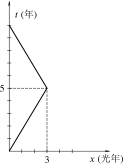
\includegraphics{figure/fig11.02}
  \caption{在地球参考系看,飞船航行的时空图}
  \label{fig:11.02}
\end{wrapfigure}
若讯号的发射者与接收者以
相对速度$ v $运动,由于多普勒效
应,发射的频次$ \nu $与接收到的频
次$ \nu ^ \prime $之间应当有以下关系:
{\setlength{\mathindent}{4em}
\begin{equation*}
  \nu ^ { \prime } = \sqrt { \frac { 1 - v / c } { 1 + v / c } \nu }
\end{equation*}}
当飞船与地球远离时,
{\setlength{\mathindent}{4em}
\begin{equation*}
  v = + \frac { 3 } { 5 } c \qquad \nu ^ { \prime } = \frac 1 2 \nu
\end{equation*}}
当飞船与地球接近时,
{\setlength{\mathindent}{4em}
\begin{equation*}
  v = - \frac { 3 } { 5 } c \qquad \nu ^ { \prime } = 2 \nu
\end{equation*}}

据此,得以下两表中的结果。注意,飞船在$ t ^ { \prime } = 4 $时转向,此
时飞船经受加速度。
\vspace{0.8em}
\begin{table}[!h]
  %\vspace{-1em}
  \caption{地球的光钟发出的脉冲读数$ t $到达飞船时,飞船上光钟的读数$ t' $}
  \label{tab:11.01}
  \centering
  %\setlength{\tabcolsep}{1.5em}
  \begin{tblr}{colsep=5pt,colspec={X[c]*{2}{|X[c]}|c*{8}{|X[c]}}}
    \toprule
    $t$  & 0 & 1 & 2        & 3   & 4 & 5   & 6 & 7   & 8 & 9   & 10 \\
    \midrule
    $t'$ & 0 & 2 & 4 (飞船转向) & 4.5 & 5 & 5.5 & 6 & 6.5 & 7 & 7.5 & 8  \\
    \bottomrule
  \end{tblr}
\end{table}
\vspace{0.8em}
\begin{table}[!h]
  %\vspace{-1em}
  \caption{飞船上光钟发出的脉冲读数$ t' $到达地球时,地球的光钟的读数$ t $}
  \label{tab:11.02}
  \centering
  %\setlength{\tabcolsep}{1.5em}
  \begin{tblr}{X[c]*{4}{|X[c]}|c*{4}{|X[c]}}
    \toprule
    $t'$ & 0 & 1 & 2 & 3 & 4 (飞船转向) & 5   & 6 & 7   & 8  \\
    \midrule
    $t$  & 0 & 2 & 4 & 6 & 8        & 8.5 & 9 & 9.5 & 10 \\
    \bottomrule
  \end{tblr}
\end{table}
\vspace{0.8em}

\example 一列火车在一平直的铁道上匀速行驶,铁道穿过
% 337.jpg
一个隧道。在静止时,火车恰好与隧道一样长。然而,现在火车
以$ v = \dfrac { 3 } { 5 } c $的速率运行。火车司机说:“隧道由于洛伦兹收缩,
比火车短,因此,火车决不可能在任一时刻全部处在隧道之中。”
隧道看守人却说:“火车因为洛伦兹收缩,比隧道短,所以火车
在某一时刻是全部处在隧道之中的。”他们谁也说服不了谁。

(1) 司机决定用实验解决这个争论。他在火车头尾两端各安
装一个定时火箭,使火车的中点与隧道中点重合时,两个火箭同
时沿竖直方向飞出。这将发生什么结果?画出这些事件的时空
图,分别用火车参考系和隧道参考系描述这些事件的先后次序。

(2) 隧道看守人也不示弱。他在隧道两端竖立巨大的定时铁
门,使得当火车中点到达隧道中点时,两门同时关上。用两种参
考系来描述这些事件的先后次序。

\solution 为了说明事件的次序,用时空图的方法最清楚

(1) 取火车为参考系$ K $,隧道为参考系$ K' $,隧道以
$ v = - \dfrac { 3 } { 5 } c $
向负x方向运动,根据式\eqref{eqn:11.04.09},二者的变换为
\begin{equation*}
  x^{\prime}=\frac{x+v t}{\sqrt{1-\dfrac{v^{2}}{c^{2}}}} \quad t^{\prime}=\frac{t+\dfrac{v}{c^{2}} x}{\sqrt{1-\dfrac{v^{2}}{c^{2}}}}
\end{equation*}
$ t ^ { \prime } $轴是
\begin{equation*}
  x ^ { \prime } = 0
\end{equation*}
即
\begin{equation*}
  x + v t = 0
\end{equation*}
为过原点、斜率为$ \dfrac { \Delta x } { \Delta t } = - \dfrac { 3 } { 5 } $的直线。同理可求得$ x ^ { \prime } $轴是过原
点,斜率为$ - \dfrac { 5 } { 3 } $的直线。如图11.3所示,$ \tg \theta = - \dfrac { 3 } { 5 } $。

% 338.jpg
\clearpage
\begin{figure}[h]
  \centering
  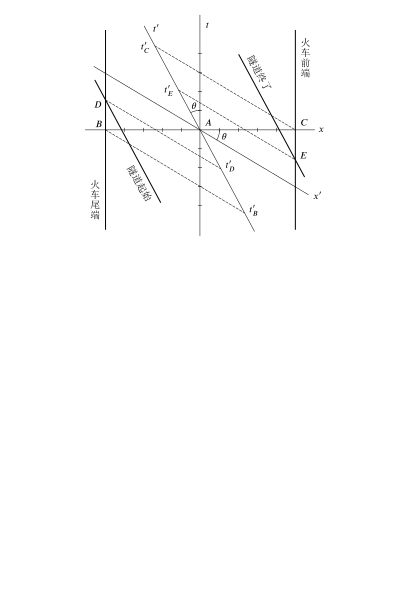
\includegraphics{figure/fig11.03}
  \caption{}
  \label{fig:11.03}
\end{figure}

\begin{center}
  \zihao{6}
  \begin{tabular}{ll}
    $ A $——火车中点与隧道中点相重合; & $ B $——火车尾端火箭爆发; \\
    $ C $——火车前端火箭爆发;     & $ D $——火车尾端进入隧道; \\
    $ E $——火车前端从隧道出来     &                  \\
  \end{tabular}
\end{center}

从时空图上很容易看清楚,虽然$ K $系的司机及$ K ^ { \prime } $系的看守都
确认:火箭是在隧道外面发射的,但各自认定的事件顺序却不
同。司机认为,事件的顺序是$ E, (A, B, C), D $,两支火箭都
是在比火车短的隧道之外同时爆发的。看守却认为,事件
的顺序
是$ B, D, A, E, C $,一个火箭爆发得太早($ t _ { B } ^ { \prime } < t _ { A } ^ { \prime } $),而另一个则
爆发得太迟($ t _ { C } ^ { \prime } < t _ { A } ^ { \prime } $),虽然火车比隧道短,但火箭却都是在外面爆
发的。

(2) 按上述同样方法作出图11.4,取隧道参考系为$ K $,火车
参考系为$ K' $,火车以$ v = \dfrac { 3 } { 5 } c $向x轴正方向运动,$ \tg \theta = \dfrac { 3 } { 5 } $。

隧道看守认为,事件的顺序是$ D, (A, B, C), E $,火车尾
端是在两门关上之前进入隧道的,火车前端是在两门关上之后试
% 339.jpg
图冲出
去的,所以火车变短与车撞铁门没有矛盾。司机认为,事
件的顺\clearpage\noindent
序是$ C, E, A, D, B $,他认为,前方铁门关得太早
($ t _ { C } ^ { \prime } < t _ { A } ^ { \prime } $) ,
发生了碰撞,而碰撞的讯号沿碰撞光锥线传播,尚未传到
火车后端,故不知撞车事件的火车后端继续行驶,使得它在关得
太迟的后方铁门落下之前进入隧道($ t _ { B } ^ { \prime } < t _ { D } ^ { \prime } $)。

\begin{figure}[h]
  \centering
  \includegraphics{figure/fig11.04}
  \caption{}
  \label{fig:11.04}
\end{figure}

\begin{center}
  \zihao{6}
  \begin{tabular}{ll}
    $ A $——火车中点与隧道中点相重合; & $ B $——隧道起始处门关上; \\
    $ C $——道终了处门关上;      & $ D $——火车尾端进入隧道; \\
    $ E $——火车前端撞上铁门      &                  \\
  \end{tabular}
\end{center}

\example 光行差问题相对论的“海市蜃楼”。不仅时间
的“先后”会变化,空间的“前后”也会变化。有时候为了表示
“绝对不可能”这种意思,我们常说:谁能看见自己脑后头的东
西的确,人眼的视角只比$ 180 $度稍大一点。所以,要想看到脑
后的东西,似乎是绝对办不到的。

根据相对论,则不尽然。

设想一条飞船,飞船前端有一个半球形的观察室。此飞船沿
正$ x $方向飞行,接受到一颗恒星发出的光讯号。在恒星为静止的

% 340.jpg
\clearpage\noindent
\begin{wrapfigure}[8]{r}{14em}
  \centering
  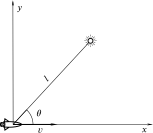
\includegraphics{figure/fig11.05}
  \caption{}
  \label{fig:11.05}
\end{wrapfigure}
参考系$ K $中,星在$ xy $平面上,讯
号来的方向与飞船的轴成$ \theta $角。
根据洛伦兹变换,在飞船为静止
参考系$ K ^ { \prime }$中,讯号来的方向角
为$ \theta ^ { \prime } $,所有$ \theta ^ { \prime } < \dfrac { \uppi } { 2 } $的恒星,在观
察室里都可以看见(图11.5)

根据式\eqref{eqn:11.04.05},取$ c = 1 $,
得
\begin{align*}
  x ^ { \prime } & = x \ch \varphi - t \sh \varphi
  \quad y ^ { \prime } = y \quad z ^ { \prime } = z \\
  t ^ { \prime } & = t \ch \varphi - x \sh \varphi
\end{align*}
其中有
\begin{equation*}
  \th ^ { - 1 } v = \varphi
\end{equation*}
设恒星距离为$ l $,则在$ x = l \cos \theta , y = l \sin \theta , t = - l $发的光,
在$ x = 0 , y = 0 , t = 0 $被接收到。所以,在$ x ^ { \prime } = 0 , y ^ { \prime } = 0 , t ^ { \prime } = 0 $接
收到的光,是在
\begin{align*}
  x ^ { \prime } & = \left( l \cos \theta \right) \ch \varphi - \left( - l \right) \sh \varphi \\
  y ^ { \prime } & = \left( l \sin \theta \right)                                              \\
  t ^ { \prime } & = \left( - l \right) \ch \varphi - \left( l \cos \theta \right) \sh \varphi
\end{align*}
发射的。

由此求得
\begin{align*}
  \tg \theta ^ { \prime } & = \frac { \Delta y ^ { \prime } } { \Delta x ^ { \prime } }             \\
                          & = \frac { l \sin \theta } { l \cos \theta \ch \varphi + l \sh \varphi }
\end{align*}
所有$ \theta ^ { \prime } < \dfrac { \uppi } { 2 } $的恒星,都观察得到,此即要求
\begin{equation*}
  \tg \theta ^ { \prime } < \infty
\end{equation*}
% 341.jpg
\begin{align*}
  \beforetext{或} l \cos \theta \ch \varphi + l \sh \varphi > 0
\end{align*}
即
\begin{equation*}
  \cos \theta > - \th \varphi
\end{equation*}
当$ v = 1 $即($ v = c $)时,$ \th \varphi = 1 $,
上式变成
\begin{equation*}
  \cos \theta > - 1
\end{equation*}
即
\begin{equation*}
  \theta < 1 8 0 ^ { \circ }
\end{equation*}
此时全部星空都可以在飞船观察室里看见。

具体地说,如果飞船的航向指向北极星,当它的速度很小
时,观察室内乘员$ A $眼前的星空景象同生活在地面上的人面向北
极星时所看到的是一样的。这时,北极星在中央,北斗、仙后、
武仙等星座环绕在它的周围\lhbrak 图\ref{fig:11.06a}\rhbrak ,南天的星不在视野之
内。

\begin{figure}[h]
  \centering
  \subfigure[\label{fig:11.06a}]{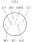
\includegraphics{figure/fig11.06a}}
  \subfigure[\label{fig:11.06b}]{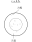
\includegraphics{figure/fig11.06b}}
  \subfigure[\label{fig:11.06c}]{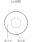
\includegraphics{figure/fig11.06c}}
  \caption{不同速度时飞船人看到的景象}
  \label{fig:11.06}
\end{figure}

飞船加快速度,当达到光速的一半时,展现在A眼前的星空
景象将大大变化了。他看到原来在北极星周围的屋都向中央聚
拢,挤到虚线圆所表示的范围之中,虚线圆外面的天狼和天蝎,
% 342.jpg
原来都是在“后”面的,现在开始进入前面\lhbrak 图\ref{fig:11.06b}\rhbrak 。

随着速度的继续增大,将有越来越多的原来在“脑后”的星
进入视野。当速度达到光速的$ 90\% $时,南天的十字座和老人星也
都能看到了\lhbrak 图\ref{fig:11.06c}\rhbrak 。如果飞船速度接近光速,则原来整个天
空中的所有恒星和星系,都无例外地“挤”到前面来了。

因此,只要运动速度足够接近光速,那么,即使原来在脑后
的东西,我们也是能看到的。这就出现一种奇怪的景象,当$ A $以
接近光的速度逃离地球时,他将看到地球就在他的航向的前侧
方;当$ A $以接近光的速度逃离太阳时,太阳也就在他的航向的前
侧方。无论他向什么方向逃,他要离开的地方总是在他的前方
其实,他看见的只不过是相对论的“海市蜃楼”。
